\documentclass[a4paper]{article}
\usepackage{graphicx}
\usepackage{xcolor}
\usepackage{url}
\usepackage{parcolumns}
\usepackage[hidelinks]{hyperref}
\usepackage{multicol}
\usepackage{outlines}
\usepackage{listings}
\usepackage{fontspec}
\lstset{basicstyle=\ttfamily,
	showstringspaces=false,
	commentstyle=\color{blue},
	keywordstyle=\color{black}
}
\newcommand{\abc}{\hfill \break}
\newcommand{\vi}{\vfill}
\newcommand{\ii}{\textit}
\newcommand{\ttt}{\texttt}
\usepackage{fancyhdr}
\usepackage{geometry}
\geometry{
	a4paper,
	total={170mm,257mm},
	left=20mm,
	top=20mm,
	bottom=39mm,
}

\setlength{\headheight}{82.70538pt}

\fancypagestyle{oida}{
	\fancyhf{}
	\fancyhead[L]{\fontsize{7.5}{7.5}htl donaustadt\\ Donaustadtstraße 45\\
		1220 Wien\\~\\ Abteilung: Informationstechnologie\\ 
	Schwerpunkt: Netzwerktechnik}
	\fancyhead[R]{
\includegraphics[scale=0.45]{images/logo.png}}

	\fancyfoot[L]{\today}
	\fancyfoot[C]{\jobname}
	\fancyfoot[R]{Seite: \thepage}
}

\begin{document}
% \bibliographystyle{plain}
\pagestyle{oida}
\subsection*{Exercise 3: 4.2.8 Lab - Configure Router-on-a-Stick Inter-VLAN Routing}
\par\noindent\rule{\textwidth}{0.4pt}

Laboratory protocol

\begin{figure}[h]
	
\includegraphics[scale=0.2]{images/mika.jpeg}
	\centering
\end{figure}

\vspace*{\fill}
\textbf{Subject:}	NWT\abc

\textbf{Class:}	3AHITN\abc

\textbf{Name:}	Stefan Fürst, Marcel Raichle\abc

\textbf{Groupname/Number} Team 7/7\abc

\textbf{Supervisor:} 	ANGE, ZIVK\abc

\textbf{Exercise dates:} 9.1.2025	\abc

\textbf{Submission date:}\abc

\abc \abc \abc \abc

\newpage
\tableofcontents

\newpage

\section{Task definition}

In this task, you will configure VLANs, trunking, and inter-VLAN routing. The objectives are to build the network, create and assign VLANs, set up 802.1Q trunking between switches, configure inter-VLAN routing on the router, and verify that inter-VLAN routing works.\abc
VLANs provide network segmentation, and communication between them requires a Layer 3 device, such as a router. The "Router-on-a-Stick" configuration allows multiple VLANs to communicate via a trunk link from the router to the switch. \abc
To begin, you will first cable the network and configure basic settings on the router and switches. This includes assigning device names, passwords, and IP addresses to the devices. Next, you will create the required VLANs on the switches and assign them to the appropriate ports. You will then configure 802.1Q trunking on switch ports to allow VLAN traffic to pass between switches and the router. \abc
On the router, you will configure sub-interfaces for each VLAN using 802.1Q encapsulation to enable inter-VLAN routing. Finally, you will test the setup by pinging between PCs, testing the connectivity and ensuring that inter-VLAN routing is functioning. You will also use the \texttt{tracert} command to verify the routing path from one PC to another.\abc
This task demonstrates VLAN creation, trunking setup, and inter-VLAN routing using the "Router-on-a-Stick" method.\footnote{This Task definition was written by ChatGPT.}

\section{Summary}

This exercise involved configuring a network with VLANs, trunking, and inter-VLAN routing using a router-on-a-stick setup. Initially, the network topology was established by cabling the devices as shown in the diagram, with routers and switches set up with basic settings such as device names, passwords, and IP addresses.\abc
After the network setup, VLANs were created on the switches, and each VLAN was assigned to the corresponding interfaces. The switches were then configured to allow VLAN traffic to pass between them by establishing 802.1Q trunk links. Trunks were configured on both switches, including the setting of the native VLAN and allowing specific VLANs to pass through.\abc
For inter-VLAN routing, the router was configured with sub-interfaces for each VLAN, ensuring that 802.1Q encapsulation was applied for proper VLAN identification. The router's interface was activated, and sub-interfaces were set with appropriate IP addresses for each VLAN, enabling communication across different VLANs.\abc
Finally, the functionality of the network was verified by performing tests from the PCs. Successful pings between the PCs and the default gateways confirmed that inter-VLAN routing was working. Additionally, the \texttt{tracert} command was used to trace the routing path between the PCs, further verifying that the routing configuration was correct.\abc
Overall, the exercise demonstrated the successful configuration of VLANs, 802.1Q trunking, and inter-VLAN routing, ensuring seamless communication between hosts in different VLANs.\footnote{This summary was written by ChatGPT.}


\newpage

\section{Complete network topology of the exercise}

\begin{figure}[h]
	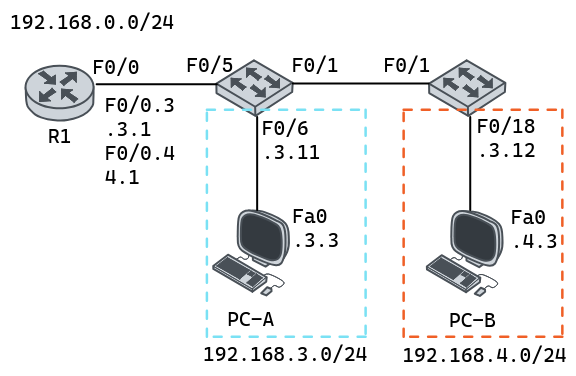
\includegraphics[scale=0.8]{images/tpologie.png}
	\centering
	\caption{Complete network topology of this exercise}
\end{figure}

\newpage

\section{Exercise Execution}
\subsection{Build the Network and Configure Basic Device Settings}
To get starteed with the 
\subsubsection{Configure basic settings for the router.}
To access the router's configuration mode, connect to the router through the console port and execute the \ii{en} and \ii{conf t} commands.\abc
The following basic settings are configured using the commands listed below: \footnote{I won't add any screenshots for the basic configuration, as this has already been covered in the last two exercises and is therefore redundant.}
\begin{lstlisting}[language=bash]
#Assign a hostname to the router
hostname R1
#Disable DNS lookup on mistyped commands
no ip domain-lookup
#setting a encrypted password to enter EXEC mode
enable secret class
#Set cisco as the password for console access and enable login
line console 0
password cisco
login
#Set cisco as VTY password and enable login
line vty 0 4
password cisco
login
#Encrypting the plaintext password
service password-encryption
#Createing a banner to warn that unauthorized access is prohibited
banner motd & Unauthorized access prohibited $
#Writeing the running config to the NVRAM
do wr mem
#Setting the clock
do clock set HH:MM:SS DAY MONTH YEAR
\end{lstlisting}

\subsubsection{Configure basic settings for each switch}
To access the router's configuration mode, connect to the switch through the console port and execute the \ii{en} and \ii{conf t} commands.\abc
The following basic settings are configured using the commands listed below:
\begin{lstlisting}[language=bash]
#Assign a hostname to the switch 1
hostname S1
#Assign a hostname to the switch 2
hostname S2
#Disable DNS lookup on mistyped commands
no ip domain-lookup
#setting a encrypted password to enter EXEC mode
enable secret class
#Set cisco as the password for console access and enable login
line console 0
password cisco
login
#Set cisco as VTY password and enable login
line vty 0 4
password cisco
login
#Encrypting the plaintext password
service password-encryption
#Createing a banner to warn that unauthorized access is prohibited
banner motd & Unauthorized access prohibited $
#Writeing the running config to the NVRAM
do wr mem
#Setting the clock
do clock set HH:MM:SS DAY MONTH YEAR
\end{lstlisting}

\subsubsection{Configure PC hosts}
To configure the PC hosts, the Settings app of each operating system was used. Under the respective network tab, the IP settings were changed from automatic to manual and filled with the information from the addressing table.
\begin{figure}[h]
	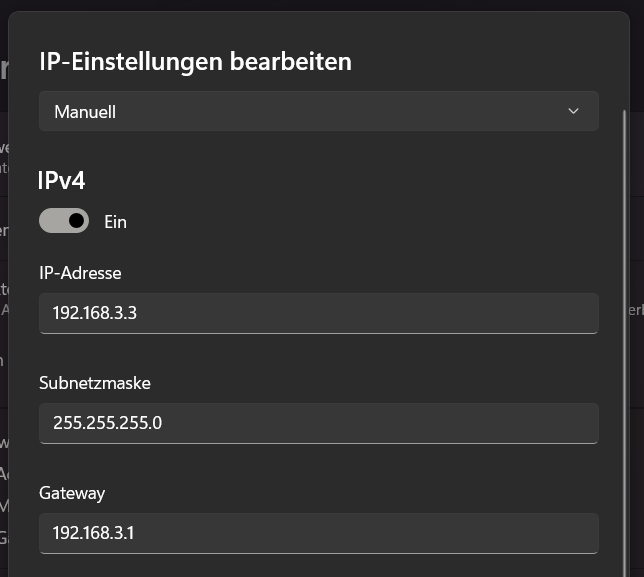
\includegraphics[scale=0.4]{images/ipconfmar.png}
	\centering
	\caption{Configure the IP settings for PC A}
\end{figure}
\begin{figure}[h]
	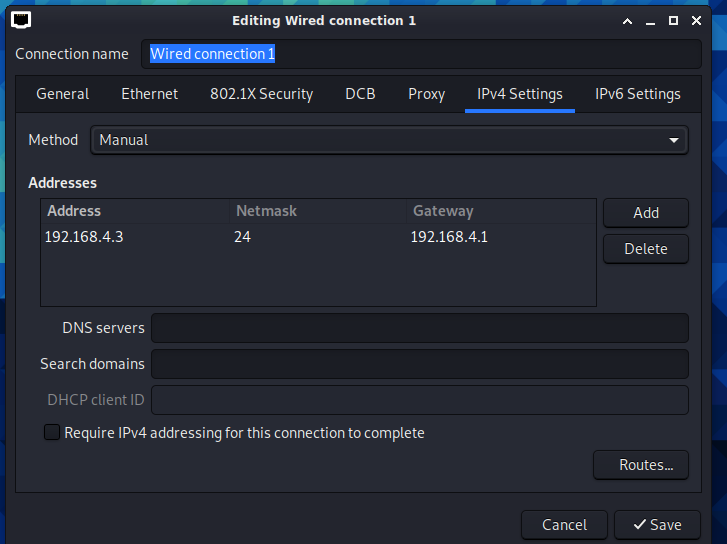
\includegraphics[scale=0.27]{images/ipconfich.png}
	\centering
	\caption{Configure the IP settings for PC B}
\end{figure}
\newpage
\subsection{Create VLANs and Assign Switch Ports}
\subsubsection{Create VLANs on both switches}
To create VLANs, the global configuration must be entered. Since the VLANs are the same on both switches, I will list the configuration only once.
\begin{lstlisting}[language=bash]
#Creating VLAN 3
vlan 3
#Setting a name of it
name Management
#Creating VLAN 4
vlan 4
#Setting a name of it
name Operations
#Creating VLAN 7
vlan 7
#Setting a name of it
name ParkingLot
#Creating VLAN 8
vlan 8
#Setting a name of it
name Native
\end{lstlisting}
To set a default gateway and an IP address for management in each VLAN, use the \ii{interface vlan <number>} command, followed by the \ii{ip address <address> <subnet\_mask>} command, and then the \ii{no shutdown} command to configure the VLAN, set its IP address, and enable it.
Lastly, the default gateway is set in global configuration mode rather than for the interface. \footnote{The commands that are the same for both S1 and S2 will only be written once from now on, and the comment above the command will indicate if there are any differences.}
\begin{lstlisting}[language=bash]
#Entering the configuration for the VLAN 3 interface
interface vlan 3
#Setting the IP address for S1
ip address 192.168.3.11 255.255.255.0
#Setting the IP address for S2
ip address 192.168.3.12 255.255.255.0
#Enabling the interface
no shutdown
#Returning to global configuration mode
exit
#Setting the default gateway
ip default-gateway 192.168.3.1
\end{lstlisting}
\subsubsection{Assign VLANs to the correct switch interfaces}
To assign all unused interfaces to the Parking Lot VLAN, the \ii{interface range} command is used to edit multiple interfaces at the same time. These interfaces are then set to access mode with \ii{switchport mode access}, assigned to the VLAN with \ii{switchport access vlan <number>}, and disabled with \ii{shutdown}.
\begin{lstlisting}[language=bash]
#Selecting the ports on S1
interface range f0/2 - 4 , f0/7 - 24 , g0/1 - 2	
#Selecting the ports on S2
interface range f0/2 - 17, f0/19 - 24 , g0/1 - 2
#Setting the interface mode to access
switchport mode access
#Setting the the Interface to access VLAN 7
switchport access vlan 7
#Disabling those interfaces
shut
#Returning to global configuration mode
exit
#Selecting Fast Ethernet port 6 (on S1)
interface f0/6
#Selecting Fast Ethernet port 18 (on S2)
interface f0/18
#Setting the interface mode to access
switchport mode access
#Setting the the Interface to access VLAN 3
switchport access vlan 3
\end{lstlisting}
The VLAN configuration can be examined using the \ii{show vlan brief} command.
\begin{figure}[h]
	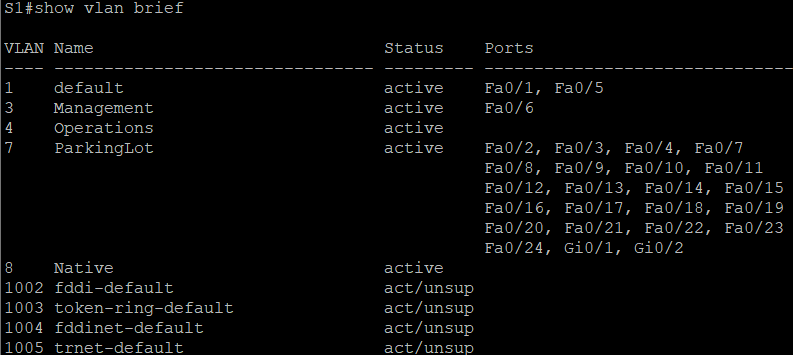
\includegraphics[scale=0.4]{images/s1_show_vlan_brief.png}
	\centering
	\caption{Examining the VLAN configuration of S1}
\end{figure}
\begin{figure}[h]
	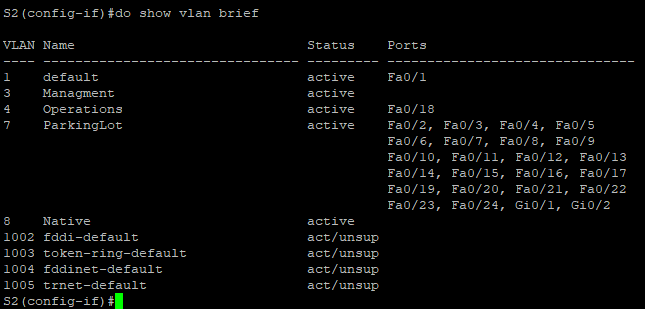
\includegraphics[scale=0.37]{images/s2_show_vlan_brief.png}
	\centering
	\caption{Examining the VLAN configuration of S2}
\end{figure}

\subsection{Configure an 802.1Q Trunk Between the Switches}

\subsubsection{Manually configure trunk interface F0/1}
To enable \ii{802.1Q} trunking, the \ii{switchport trunk encapsulation dot1q} command must be used so that the \ii{switchport mode trunk} command works, as the interface's trunk encapsulation is set to "Auto" by default.

\begin{figure}[h]
	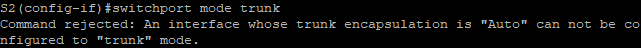
\includegraphics[scale=0.55]{images/upsi.png}
	\centering
	\caption{The \ii{switchport mode trunk} command does not work because the encapsulation is set to "Auto".}
\end{figure}
\begin{lstlisting}[language=bash]
#Entering configuration for FastEthernet 0/1.
interface f0/1	
Changing the encapsulation mode to 802.1Q.
switchport trunk encapsulation dot1q
#Changing the port mode to trunk
switchport mode trunk
#Setting the the native VLAN
switchport trunk native vlan 8
#Setting the allowed VLANs for the trunk.
switchport trunk allowed vlan 3,4,8
\end{lstlisting}
To verify this configuration, the \ii{show int trunk} command is used.
\begin{figure}[h]
	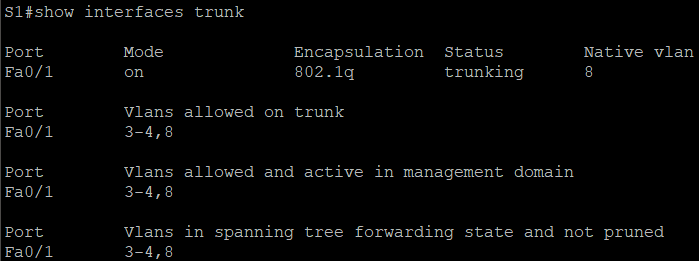
\includegraphics[scale=0.55]{images/s1_show_trunk.png}
	\centering
	\caption{Verifying the trunk configuration of S1.}
\end{figure}
\begin{figure}[h]
	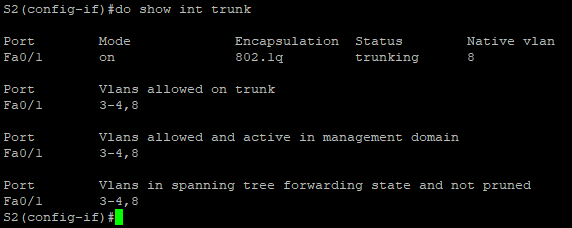
\includegraphics[scale=0.55]{images/s2_show_trunk.png}
	\centering
	\caption{Verifying the trunk configuration of S2.}
\end{figure}
\newpage
\subsubsection{Manually configure S1’s trunk interface F0/5}
The trunk on interface FastEthernet 0/5 is the trunk with the router, which is configured like any other trunk using the following commands:
\begin{lstlisting}
interface f0/5
switchport mode trunk
switchport trunk native vlan 8
switchport trunk allowed vlan 3,4,8
\end{lstlisting}
If the \ii{show interfaces vlan brief} command is run again, FastEthernet 0/5 won't show, since the status of the interface on the router is set to administratively down.
\begin{figure}[!htbp]
	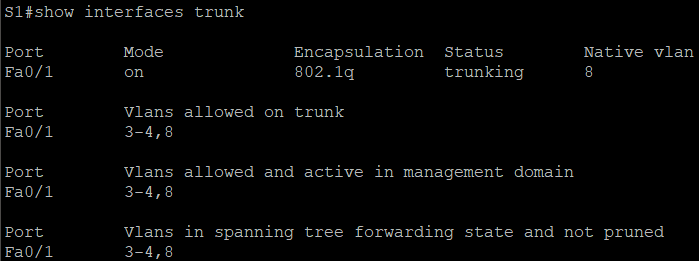
\includegraphics[scale=0.55]{images/s1_show_trunk.png}
	\centering
	\caption{FastEthernet 0/5 is missing from the list.}
\end{figure}
\subsection{Configure Inter-VLAN Routing on the Router}
To configure inter-VLAN routing via Router on a Stick, subinterfaces are used on the router. First, the desired interface must be activated by using the \ii{no shutdown} command. In this case, the interface FastEthernet 0/0 was used.
\begin{lstlisting}[language=bash]
#Activating the interface
interface f0/0	
no shut
\end{lstlisting}
To enable inter-VLAN routing, subinterfaces must be created for each VLAN, the encapsulation must be set to \ii{802.1Q}, and an IP address and description must be configured as well.
\begin{lstlisting}[language=bash]
#Creating a new subinterface for VLAN 3
interface f0/0.3
#Giving the VLAN a description
description Management Network
#Setting the encapsulation to 802.1Q
encapsulation dot1q 3
#Setting the IP address of the interface
ip address 192.168.3.1 255.255.255.0
#Setting up the subinterface for VLAN 4
interface f0/0.4
description Operations Network
encapsulation dot1q 4
ip address 192.168.4.1 255.255.255.0
#Setting up the subinterface for VLAN 4
interface f0/0.8
description Native VLAN
#Making it the native VLAN
encapsulation dot1q 8 native
\end{lstlisting}
\newpage
The configuration of the subinterfaces can be examined by issuing the \ii{show interfaces brief} command.
\begin{figure}[!htbp]
	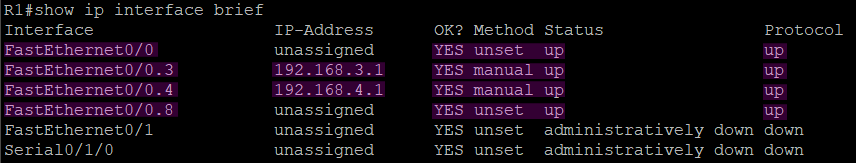
\includegraphics[scale=0.55]{images/R1_show_int_brief.png}
	\centering
	\caption{Examining the configuration of the interfaces on R1.}
\end{figure}
\subsection{Verify Inter-VLAN Routing is Working}
To verify if inter-VLAN routing is configured correctly, three pings will be executed.
\begin{enumerate}
	\item Ping from PC-A to its default gateway.
	\item Ping from PC-A to PC-B
	\item Ping from PC-A to S2
\end{enumerate}
\begin{figure}[!htbp]
	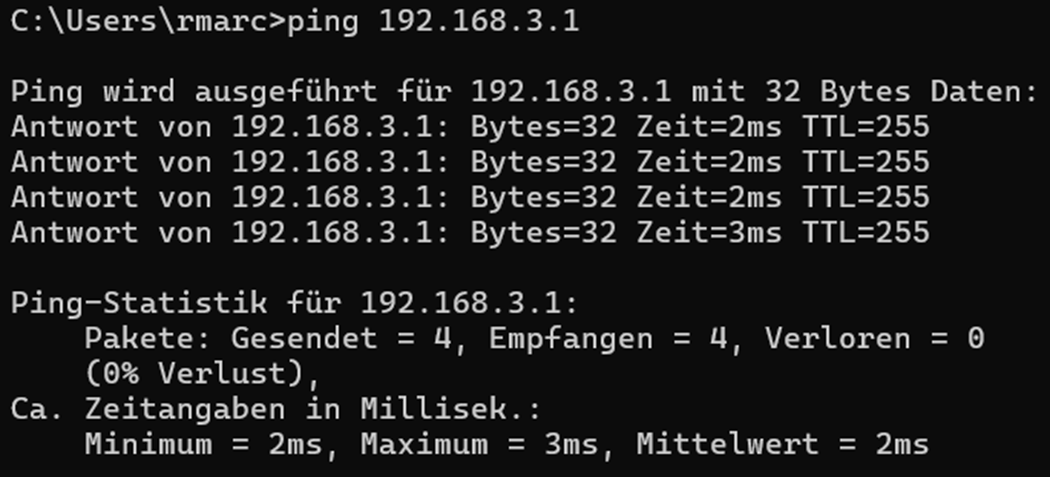
\includegraphics[scale=0.55]{images/PC_A_ping_Gateway.png}
	\centering
	\caption{Pinging the default gateway of PC-A.}
\end{figure}
\begin{figure}[!htbp]
	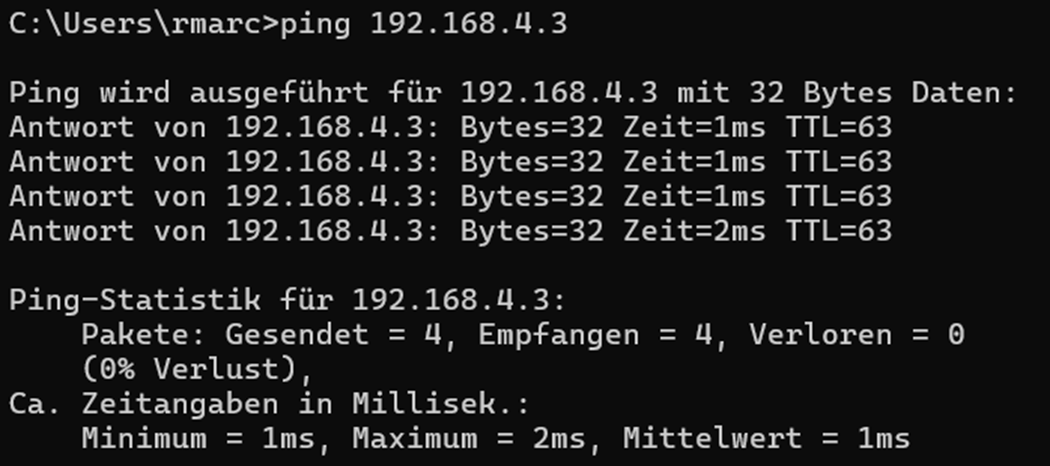
\includegraphics[scale=0.55]{images/PC_A_ping_PC_B.png}
	\centering
	\caption{Pinging PC-B from PC-A.}
\end{figure}\newpage
\begin{figure}[!htbp]
	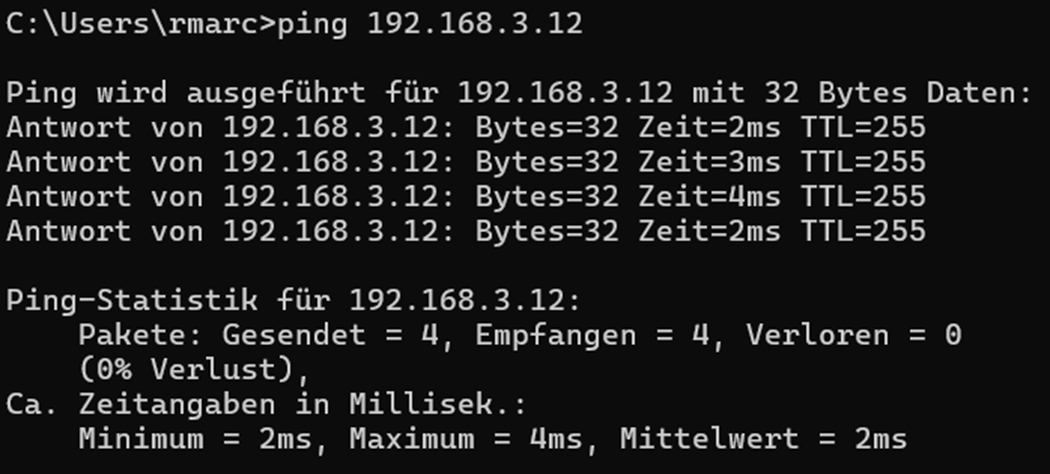
\includegraphics[scale=0.55]{images/PC_A_ping_S2.png}
	\centering
	\caption{Pinging S2 from PC-A.}
\end{figure}\abc
Additionally, the \ii{tracert} command can be used to show the route of the communication.
\begin{figure}[!htbp]
	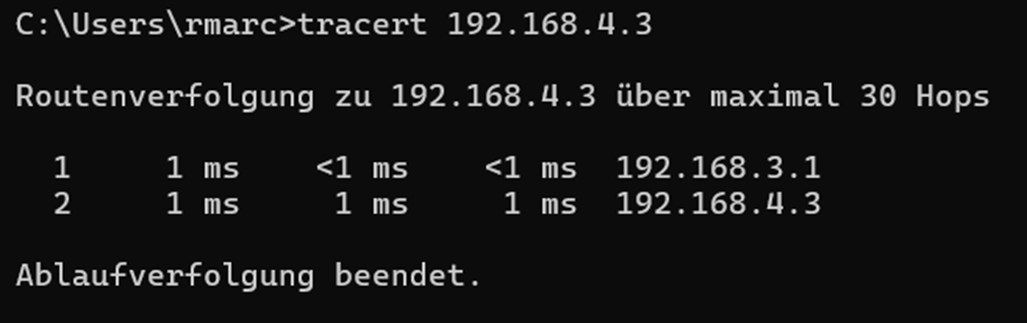
\includegraphics[scale=0.55]{images/PC-A_tracert.png}
	\centering
	\caption{Using the \ii{tracert} command from PC-A to PC-B.}
\end{figure}\abc
The output from the command tells us that the first hop was to FastEthernet 0/0 on R1, and then it went straight to PC-B for the second hop.\abc
Lastly, the routing table of R1 can be displayed using the \ii{show ip route} command.
Routing table from R1.
\begin{figure}[!htbp]
	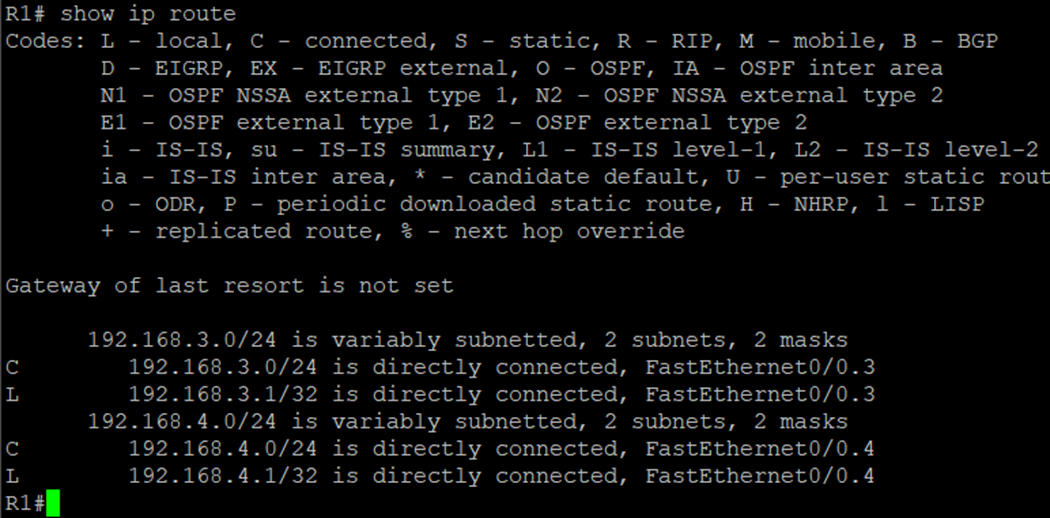
\includegraphics[scale=0.55]{images/R1_routing_table.png}
	\centering
	\caption{Routing table from R1.}
\end{figure}\abc
\newpage
\section{Complete configuration files}
\begin{multicols}{2}
	\begin{lstlisting}[language=bash]
#Router configuration
version 15.1
service timestamps debug datetime msec
service timestamps log datetime msec
service password-encryption
!
hostname R1
!
boot-start-marker
boot-end-marker
!
enable secret 5\
$1$lggJ$sTcxYQPrT9zZuLSp1CZzT/
!
no aaa new-model
!
memory-size iomem 15
crypto pki token default removal \
timeout 0
!
dot11 syslog
ip source-route
!
ip cef
no ip domain lookup
no ipv6 cef
!
multilink bundle-name authenticated
!
voice-card 0
!
license udi pid CISCO2801 sn\
FCZ1013228P
!
redundancy
!
interface FastEthernet0/0
 no ip address
 duplex auto
 speed auto
!
interface FastEthernet0/0.3
 description Management Network
 encapsulation dot1Q 3
 ip address 192.168.3.1 255.255.255.0
!
interface FastEthernet0/0.4
 description Operations Network
 encapsulation dot1Q 4
 ip address 192.168.4.1 255.255.255.0
!
interface FastEthernet0/0.8
 description Native VLAN
 encapsulation dot1Q 8 native
!
interface FastEthernet0/1
 no ip address
 shutdown
 duplex auto
 speed auto
!
interface Serial0/1/0
 no ip address
 shutdown
 clock rate 125000
!
interface Serial0/1/1
 no ip address
 shutdown
 clock rate 125000
!
ip forward-protocol nd
!
no ip http server
no ip http secure-server
!
control-plane
!
mgcp profile default
!
banner motd ^C Unauthorized access\
prohibited ^C
!
line con 0
 password 7 110A1016141D
 login
line aux 0
line vty 0 4
 password 7 121A0C041104
 login
 transport input all
!
scheduler allocate 20000 1000
end	

#Switch 1 Configuration
version 12.2
no service pad
service timestamps debug datetime msec
service timestamps log datetime msec
service password-encryption
!
hostname S1
!
boot-start-marker
boot-end-marker
!
enable secret 5\
$1$ZCk5$4NKyGg0LUDOslqtw/ANG51
!
no aaa new-model
system mtu routing 1500
no ip domain-lookup
!
crypto pki trustpoint\
TP-self-signed-1457337728
 enrollment selfsigned
 subject-name\
 cn=IOS-Self-Signed-Certificate-1457337728
 revocation-check none
 rsakeypair TP-self-signed-1457337728
!
crypto pki certificate chain\
TP-self-signed-1457337728
 certificate self-signed 01
 3082023B 308201A4 A0030201
02020101 300D0609 2A864886
F70D0101 04050030 31312F30
2D060355 04031326 494F532D
53656C66 2D536967 6E65642D
43657274 69666963 6174652D
31343537 33333737 3238301E
170D3933 30333031 30303138
32315A17 0D323030 31303130
30303030 305A3031 312F302D
06035504 03132649 4F532D53
656C662D 5369676E 65642D43
65727469 66696361 74652D31
34353733 33373732 3830819F
300D0609 2A864886 F70D0101
01050003 818D0030 81890281
8100F363 914ECD52 C8DFE7BF
E1FDD4DB 171AA606 16A71AC2
D401FA7F F5CFE691 45BB5E79
CBF759F0 7724D622 B04A32BE
BC044A17 A369E07D E0F0B492
FF9E7CEF 27AE3320 D462EF45
7AF981C6 E746BF0F 737A055D
A67157BF 008E8555 2551DB07
51897F97 99C4F954 312F317F
2B6006BD 88A89010 71EBE4D9
D8DDD2F0 36D4B8E9 E6AF0203
010001A3 63306130 0F060355
1D130101 FF040530 030101FF
300E0603 551D1104 07300582
0353312E 301F0603 551D2304
18301680 14D059C8 2A2AD3B9
D57B4473 19691D50 FB794121
18301D06 03551D0E 04160414
D059C82A 2AD3B9D5 7B447319
691D50FB 79412118 300D0609
2A864886 F70D0101 04050003
8181001C 7DDDAB6A AC024F44
B706ABF7 558E8C8E 2FCE91CB
35B40292 5D680840 7B7E3BCB
F2092E64 8D4BF6F0 FA7943F1
E7A61AAE 309A4FAF 3B6B281B
12ECA429 B9D26C09 BB12EB98
EE96A54F 0726E75F 5C5B7710
B6949F5A 41541A49 0AADA7A1
484AEB84 132729B0 C86D5D36
36804CAE BBFB8CE7 D6BE527C
048BD94B EB3F97D6 4EC534
  quit
!
spanning-tree mode pvst
spanning-tree extend system-id
!
vlan internal allocation policy\
ascending
!
interface FastEthernet0/1
 switchport trunk allowed vlan 3,4,8
 switchport trunk native vlan 8
 switchport mode trunk
!
interface FastEthernet0/2
 switchport access vlan 7
 switchport mode access
 shutdown
!
interface FastEthernet0/3
 switchport access vlan 7
 switchport mode access
 shutdown
!
interface FastEthernet0/4
 switchport access vlan 7
 switchport mode access
 shutdown
!
interface FastEthernet0/5
 switchport trunk allowed vlan 3,4,8
 switchport trunk native vlan 8
 switchport mode trunk
!
interface FastEthernet0/6
 switchport access vlan 3
 switchport mode access
!
interface FastEthernet0/7
 switchport access vlan 7
 switchport mode access
 shutdown
!
interface FastEthernet0/8
 switchport access vlan 7
 switchport mode access
 shutdown
!
interface FastEthernet0/9
 switchport access vlan 7
 switchport mode access
 shutdown
!
interface FastEthernet0/10
 switchport access vlan 7
 switchport mode access
 shutdown
!
interface FastEthernet0/11
 switchport access vlan 7
 switchport mode access
 shutdown
!
interface FastEthernet0/12
 switchport access vlan 7
 switchport mode access
 shutdown
!
interface FastEthernet0/13
 switchport access vlan 7
 switchport mode access
 shutdown
!
interface FastEthernet0/14
 switchport access vlan 7
 switchport mode access
 shutdown
!
interface FastEthernet0/15
 switchport access vlan 7
 switchport mode access
 shutdown
!
interface FastEthernet0/16
 switchport access vlan 7
 switchport mode access
 shutdown
!
interface FastEthernet0/17
 switchport access vlan 7
 switchport mode access
 shutdown
!
interface FastEthernet0/18
 switchport access vlan 7
 switchport mode access
 shutdown
!
interface FastEthernet0/19
 switchport access vlan 7
 switchport mode access
 shutdown
!
interface FastEthernet0/20
 switchport access vlan 7
 switchport mode access
 shutdown
!
interface FastEthernet0/21
 switchport access vlan 7
 switchport mode access
 shutdown
!
interface FastEthernet0/22
 switchport access vlan 7
 switchport mode access
 shutdown
!
interface FastEthernet0/23
 switchport access vlan 7
 switchport mode access
 shutdown
!
interface FastEthernet0/24
 switchport access vlan 7
 switchport mode access
 shutdown
!
interface GigabitEthernet0/1
 switchport access vlan 7
 switchport mode access
 shutdown
!
interface GigabitEthernet0/2
 switchport access vlan 7
 switchport mode access
 shutdown
!
interface Vlan1
 no ip address
 shutdown
!
interface Vlan3
 ip address 192.168.3.12 255.255.255.0
!
ip default-gateway 192.168.3.1
ip classless
ip http server
ip http secure-server
!
banner motd ^C Unauthorized access \
is strictly prohibited ^C
!
line con 0
 password 7 1511021F0725
 logging synchronous
 login
line vty 0 4
 password 7 05080F1C2243
 logging synchronous
 login
line vty 5 15
 password 7 05080F1C2243
 logging synchronous
 login
!
end
#Switch 2 Configuration
version 12.2
no service pad
service timestamps debug datetime msec
service timestamps log datetime msec
service password-encryption
!
hostname S2
!
boot-start-marker
boot-end-marker
!
enable secret 5\
$1$ZCk5$4NKyGg0LUDOslqtw/ANG51
!
no aaa new-model
system mtu routing 1500
no ip domain-lookup
!
crypto pki trustpoint\
TP-self-signed-1457337728
 enrollment selfsigned
 subject-name\
 cn=IOS-Self-Signed-Certificate-1457337728
 revocation-check none
 rsakeypair TP-self-signed-1457337728
!
crypto pki certificate chain\
TP-self-signed-1457337728
 certificate self-signed 01
 3082023B 308201A4 A0030201
02020101 300D0609 2A864886
F70D0101 04050030 31312F30
2D060355 04031326 494F532D
53656C66 2D536967 6E65642D
43657274 69666963 6174652D
31343537 33333737 3238301E
170D3933 30333031 30303138
32315A17 0D323030 31303130
30303030 305A3031 312F302D
06035504 03132649 4F532D53
656C662D 5369676E 65642D43
65727469 66696361 74652D31
34353733 33373732 3830819F
300D0609 2A864886 F70D0101
01050003 818D0030 81890281
8100F363 914ECD52 C8DFE7BF
E1FDD4DB 171AA606 16A71AC2
D401FA7F F5CFE691 45BB5E79
CBF759F0 7724D622 B04A32BE
BC044A17 A369E07D E0F0B492
FF9E7CEF 27AE3320 D462EF45
7AF981C6 E746BF0F 737A055D
A67157BF 008E8555 2551DB07
51897F97 99C4F954 312F317F
2B6006BD 88A89010 71EBE4D9
D8DDD2F0 36D4B8E9 E6AF0203
010001A3 63306130 0F060355
1D130101 FF040530 030101FF
300E0603 551D1104 07300582
0353312E 301F0603 551D2304
18301680 14D059C8 2A2AD3B9
D57B4473 19691D50 FB794121
18301D06 03551D0E 04160414
D059C82A 2AD3B9D5 7B447319
691D50FB 79412118 300D0609
2A864886 F70D0101 04050003
8181001C 7DDDAB6A AC024F44
B706ABF7 558E8C8E 2FCE91CB
35B40292 5D680840 7B7E3BCB
F2092E64 8D4BF6F0 FA7943F1
E7A61AAE 309A4FAF 3B6B281B
12ECA429 B9D26C09 BB12EB98
EE96A54F 0726E75F 5C5B7710
B6949F5A 41541A49 0AADA7A1
484AEB84 132729B0 C86D5D36
36804CAE BBFB8CE7 D6BE527C
048BD94B EB3F97D6 4EC534
  quit
!
spanning-tree mode pvst
spanning-tree extend system-id
!
vlan internal allocation policy\
ascending
!
interface FastEthernet0/1
 switchport trunk encapsulation dot1q
 switchport trunk native vlan 8
 switchport trunk allowed vlan 3,4,8
 switchport mode trunk
!
interface FastEthernet0/2
 switchport access vlan 7
 switchport mode access
 shutdown
!
interface FastEthernet0/3
 switchport access vlan 7
 switchport mode access
 shutdown
!
interface FastEthernet0/4
 switchport access vlan 7
 switchport mode access
 shutdown
!
interface FastEthernet0/5
 switchport access vlan 7
 switchport trunk encapsulation dot1q
 switchport trunk native vlan 8
 switchport trunk allowed vlan 3,4,8
 switchport mode trunk
 shutdown
!
interface FastEthernet0/6
 switchport access vlan 7
 switchport mode access
 shutdown
!
interface FastEthernet0/7
 switchport access vlan 7
 switchport mode access
 shutdown
!
interface FastEthernet0/8
 switchport access vlan 7
 switchport mode access
 shutdown
!
interface FastEthernet0/9
 switchport access vlan 7
 switchport mode access
 shutdown
!
interface FastEthernet0/10
 switchport access vlan 7
 switchport mode access
 shutdown
!
interface FastEthernet0/11
 switchport access vlan 7
 switchport mode access
 shutdown
!
interface FastEthernet0/12
 switchport access vlan 7
 switchport mode access
 shutdown
!
interface FastEthernet0/13
 switchport access vlan 7
 switchport mode access
 shutdown
!
interface FastEthernet0/14
 switchport access vlan 7
 switchport mode access
 shutdown
!
interface FastEthernet0/15
 switchport access vlan 7
 switchport mode access
 shutdown
!
interface FastEthernet0/16
 switchport access vlan 7
 switchport mode access
 shutdown
!
interface FastEthernet0/17
 switchport access vlan 7
 switchport mode access
 shutdown
!
interface FastEthernet0/18
 switchport access vlan 4
 switchport mode access
!
interface FastEthernet0/19
 switchport access vlan 7
 switchport mode access
 shutdown
!
interface FastEthernet0/20
 switchport access vlan 7
 switchport mode access
 shutdown
!
interface FastEthernet0/21
 switchport access vlan 7
 switchport mode access
 shutdown
!
interface FastEthernet0/22
 switchport access vlan 7
 switchport mode access
 shutdown
!
interface FastEthernet0/23
 switchport access vlan 7
 switchport mode access
 shutdown
!
interface FastEthernet0/24
 switchport access vlan 7
 switchport mode access
 shutdown
!
interface GigabitEthernet0/1
 switchport access vlan 7
 switchport mode access
 shutdown
!
interface GigabitEthernet0/2
 switchport access vlan 7
 switchport mode access
 shutdown
!
interface Vlan1
 no ip address
 shutdown
!
interface Vlan3
 ip address 192.168.3.12 255.255.255.0
!
ip default-gateway 192.168.3.1
ip classless
ip http server
ip http secure-server
!
banner motd ^C Unauthorized access \
is strictly prohibited ^C
!
line con 0
 password 7 1511021F0725
 logging synchronous
 login
line vty 0 4
 password 7 05080F1C2243
 logging synchronous
 login
line vty 5 15
 password 7 05080F1C2243
 logging synchronous
 login
!
end
	\end{lstlisting}
\end{multicols}
% \newpage
% \section{References}
% \bibliography{quellen}
\newpage
\section{List of figures}

\listoffigures

\end{document}
